%%%%%%%%%%%%%%%%%%%%%%%%%%%%%%%%%%%%%%%%%%%%%%%%%%%%%%%%%%%%%%%%%%%%%%%%%%%%%%%%%%%%%%%%%%%%%%%%%
%
% TeX file ins-and-outs-gaiadr2.tex
% Uses: beamer.cls
% Last Updated:  2019.05.03
% First Created: 2019.04.26
%
% Title: The ins and out of Gaia DR2
%
% Description: Spitzer Lectures series 2019, Princeton University, May 2019
%
%%%%%%%%%%%%%%%%%%%%%%%%%%%%%%%%%%%%%%%%%%%%%%%%%%%%%%%%%%%%%%%%%%%%%%%%%%%%%%%%%%%%%%%%%%%%%%%%%

\documentclass[smaller, aspectratio=169]{beamer}

\usepackage{times,amsmath,graphicx,marvosym}
\usepackage{tikz}
\usepackage{animate}
\usepackage{colortbl}
\usetikzlibrary{arrows.meta,shapes,calc,shadows,backgrounds}
\usetheme{lightbare169}

\hypersetup{pdftitle={The ins and out of Gaia DR2},
  pdfsubject={Spitzer Lectures series 2019, Princeton University, May 2019}, colorlinks=true,
pdfauthor={Anthony Brown}}

\tikzstyle{flow}=[-{Stealth[round]}, thick, shorten >=3pt, shorten <=3pt]
\tikzstyle{flowboth}=[{Stealth[round]}-{Stealth[round]}, thick, shorten >=3pt, shorten <=3pt]

\setbeamercovered{invisible}

\graphicspath{ {./Images/} {/home/brown/Gaia/Presentation/Images/} }

\newcommand\gdrone{Gaia~DR1}
\newcommand\gdrtwo{Gaia~DR2}
\newcommand\hip{Hipparcos}
\newcommand\tyctwo{Tycho-2}
\newcommand\tyc{Tycho}
\input{/home/brown/Gaia/Presentation/GaiaDR2OverviewSlides/dr2stats}

\newcommand\llslides{\href{https://www.cosmos.esa.int/documents/29201/1770596/Lindegren_GaiaDR2_Astrometry_extended.pdf/1ebddb25-f010-6437-cb14-0e360e2d9f09}{Lindegren
et al.\ slide set}}

\title[Spitzer Lectures May 2019]{The ins and outs of Gaia DR2}
\author{Anthony Brown}
\institute{Leiden Observatory, Leiden University\\\texttt{brown@strw.leidenuniv.nl}}

\begin{document}
\logos{
}

%\begin{frame}
%  \titlepage
%\end{frame}

\setbeamercolor{background canvas}{bg=black}
\begin{emptyframe}{Title page}
  \hglue-0.57truecm
  \begin{tikzpicture}
    \node (fig) at (current page)
    {\includegraphics[width=15.9cm]{GaiaSky/GaiaDR2/ESA-PR/Gaia_s_sky_in_colour.jpg}};
      \node at ($(fig.south east)+(-0.3,0)$) [anchor=north east, font=\sf\tiny, color=white] {ESA/Gaia/DPAC};
      \node at ($(fig.south west)+(0.5,2.5)$) [anchor=south west, rotate=-45]
      {\includegraphics[height=1.8cm]{Promotion/ArtistsImpression2013.png}};
      \node (title) at ($(current page.north)+(0,-1.0)$) [anchor=north, text width=\textwidth, font=\Huge, text badly centered] {
        \structure{\color{GaiaRed}\inserttitle}
      };
      \node (author) at ($(title.south)+(0,-0.5)$) [anchor=north, text width=\textwidth, font=\Large,
      text badly centered, color=white] {\insertauthor};
      \node (institute) at (author.south) [anchor=north, text width=\textwidth, font=\large, text
      badly centered, color=white] {\insertinstitute};
  \end{tikzpicture}
\end{emptyframe}
\setbeamercolor{background canvas}{bg=white}
%
%%%%%%%%%%%%%%%%%%%%%%%%%%%%%%%%%%%%%%%%%%%%%%%%%%%%%%%%%%%%%%%%%%%%%%%%%%%%%
%
\begin{agaframe}{Credits}
  \centering
  {Most of the material in these slides is from the papers in the\\
  \href{https://www.aanda.org/component/toc/?task=topic&id=922}{Gaia DR2 A\&A special issue}\\ and
  from the\\ \llslides\ `Gaia DR2 astrometry'}
\end{agaframe}
%
\input{/home/brown/Gaia/Presentation/GaiaTalkBuildingBlocks/GaiaDR2Contents/dr2-resources-image}
%
%%%%%%%%%%%%%%%%%%%%%%%%%%%%%%%%%%%%%%%%%%%%%%%%%%%%%%%%%%%%%%%%%%%%%%%%%%%%%
%
\begin{agaframe}[1-2]{What is there besides astrometry, radial velocity, and photometry?}
  \only<1>{
    \begin{tikzpicture}
      \node (fig) {\includegraphics[height=7.0cm]{GaiaDR2/Contents/GaiaDR2-Magnitude-Distribution.pdf}};
      \node (gcrf) at ($(fig.north east)+(0.2,-1.8)$) [text width=3cm, text badly ragged,
      font=\small]
      {\textbf{Gaia-CRF2}: First optical reference frame based solely on extragalactic sources};
      \draw[flow] ($(gcrf.south west)+(0.1,0.2)$) -- ++(210:1.3cm);
    \end{tikzpicture}
  }
  \only<2>{
    \begin{itemize}
      \item Gaia Celestial Reference Frame
        \begin{itemize}
          \item Materialized by $\sim 557$ thousand QSOs identified from ALLWise
          \item Aligned to ICRF-3 through subset of $2820$ QSOs
        \end{itemize}
      \item Astrophysical parameters for stars at $G\leq17$
        \begin{itemize}
          \item \teff, $\sim 161$ million
          \item $A_G$ and $E(\gbp-\grp)$, $\sim 88$ million
          \item Radius and bolometric luminosity, $\sim77$ million
        \end{itemize}
      \item Variability information
        \begin{itemize}
          \item Photometric time series for $\sim551$ thousand sources identified as variable
            \begin{itemize}
              \item NOTE: source not explicitly listed as VARIABLE in Gaia DR2 is not necessarily
                constant
            \end{itemize}
          \item Classification for $\sim364$ thousand sources
            \begin{itemize}
              \item RRL, LPV, Cep, $\delta$ Sct, SX Phe
            \end{itemize}
          \item Detailed characterization for $\sim391$ thousand sources
            \begin{itemize}
              \item RRL, Cep, LPV, rotation modulation variables, short time scale variables
            \end{itemize}
        \end{itemize}
      \item Astrometric and photometric time series for $\sim14$ thousand minor planets
    \end{itemize}
  }
\end{agaframe}
%
%%%%%%%%%%%%%%%%%%%%%%%%%%%%%%%%%%%%%%%%%%%%%%%%%%%%%%%%%%%%%%%%%%%%%%%%%%%%%
%
\setbeamercolor{background canvas}{bg=black}
\begin{emptyframe}[1-3]{The Gaia DR2 Sky}
  \only<1>{
    \hglue-0.57truecm
    \begin{tikzpicture}
      \node (fig) at (current page)
      {\includegraphics[width=15.9cm]{GaiaSky/GaiaDR2/ESA-PR/GDR2_logdens_hammer_transparent_2000x1000.png}};
      \node at ($(fig.south east)+(-0.3,0)$) [anchor=north east, font=\sf\tiny, color=white] {ESA/Gaia/DPAC};
    \end{tikzpicture}
  }
  \only<2-3>{
    \hglue-0.57truecm
    \begin{tikzpicture}
      \node (fig) at (current page)
      {\includegraphics[width=15.9cm]{GaiaSky/GaiaDR2/02int07_fluxRGB_hammer_4000x2000_rescaled.png}};
      \node at ($(fig.south east)+(-0.3,0)$) [anchor=north east, font=\sf\tiny, color=white] {ESA/Gaia/DPAC};
      \only<3>{
        \node at (fig)
        {\includegraphics[height=6cm]{GaiaSky/GaiaDR2/Zooms/ESA_Gaia_DR2_flux_Ophiuchus_1000x750.png}};
      }
    \end{tikzpicture}
  }
\end{emptyframe}
\setbeamercolor{background canvas}{bg=white}
%
%%%%%%%%%%%%%%%%%%%%%%%%%%%%%%%%%%%%%%%%%%%%%%%%%%%%%%%%%%%%%%%%%%%%%%%%%%%%%
%
\begin{agaframe}[1-2]{Gaia DR2 spatial resolution}
  \begin{tikzpicture}
    \node (figa) {\includegraphics[height=4cm]{GaiaDR2/Contents/source_pairs_dense_field.pdf}};
    \only<1>{
      \node (figb) at ($(figa.north east)+(2.5,0)$) [anchor=north west]
      {\includegraphics[height=6cm]{GaiaDR2Science/ZiegerEtAl_gaia_recovery_heatmap.pdf}};
      \node at ($(figb.south east)+(0,0)$) [anchor=north east, font=\tiny]{
        \href{https://doi.org/10.3847/1538-3881/aad80a}{Ziegler et al.\ 2018}
      };
    }
    \only<2>{
      \node (figb) at ($(figa.north east)+(1.5,0)$) [anchor=north west]
      {\includegraphics[height=5cm]{GaiaDR2Science/GlobularClusters/DeBoerEtAl-ngc1904_profile_tie.png}};
      \node at ($(figb.south east)+(0,0)$) [anchor=north east, font=\tiny]{
        \href{https://doi.org/10.1093/mnras/stz651}{de Boer et al.\ 2019}
      };
    }
    \node at ($(figa.north east)+(0,-0.5)$) [fill=white, font=\tiny]{
      \href{https://doi.org/10.1051/0004-6361/201833234}{Arenou et al.\ 2018}
    };
    \node at (figa.south west) [anchor=north west, text width=9cm, text badly ragged] {
      \begin{itemize}
        \item Angular resolution limited to $0.4$--$0.5$ arcsec
          \begin{itemize}
            \item significantly better than all existing ground-based surveys
          \end{itemize}
        \item Will get better in later data releases
          \begin{itemize}
            \item currently no treatment of crowded sources, including binaries that are in
              principle resolved by Gaia
          \end{itemize}
    \end{itemize}};
  \end{tikzpicture}
\end{agaframe}
%
%%%%%%%%%%%%%%%%%%%%%%%%%%%%%%%%%%%%%%%%%%%%%%%%%%%%%%%%%%%%%%%%%%%%%%%%%%%%%
%
\begin{agaframe}{Gaia DR2 astrometry: uncertainties and systematic errors}
  \begin{tikzpicture}
    \node (fig) {\includegraphics[height=5cm]{UseOfGaiaAstrometry/qso-parallaxes-DR2-hist.pdf}};
    \node at ($(fig.south)+(-0.5,-1)$) [anchor=east, font=\tiny] {Images:
    \href{https://doi.org/10.1051/0004-6361/201832727}{Lindegren et al. (2018)}};
    \node at ($(fig.north)+(0.2,-0.2)$) [anchor=south, font=\scriptsize] {QSO parallaxes};
    \node at ($(fig.north east)+(0,0.8)$) [anchor=north west, text width=8.5cm, text badly ragged] {
      \begin{itemize}
        \item Uncertainties are nearly Gaussian
          \begin{itemize}
            \item NOTE: uncertainties on the astrometric parameters are correlated
          \end{itemize}
        \item Dependencies on celestial position, magnitude, colour
        \item Systematic errors are present
          \begin{itemize}
            \item non-zero mean of Gaussian uncertainty
            \item dependencies on celestial position, magnitude, colour
            \item spatially correlated
          \end{itemize}
      \end{itemize}
    };
    \node (lmc) at ($(fig.south east)+(3.5,2.3)$) [anchor=north west]
    {\includegraphics[height=4.0cm]{GaiaDR2/Contents/lmcPlxMapLabelled.pdf}};
    \node at ($(lmc.south west)+(0,1)$) [anchor=south east, text width=3cm, text badly ragged, font=\scriptsize] {Median
    parallax LMC region};
  \end{tikzpicture}
\end{agaframe}
%
%%%%%%%%%%%%%%%%%%%%%%%%%%%%%%%%%%%%%%%%%%%%%%%%%%%%%%%%%%%%%%%%%%%%%%%%%%%%%
%
\begin{agaframe}[1-2]{Random and systematic errors}
  \only<1>{
    A useful model for the total (external) error in parallax for source $i$ is
    \begin{equation}
      \varpi^\mathrm{DR2}_i-\varpi^\mathrm{true}_i = r_i + s(\alpha, \delta, G, C, \dots)
    \end{equation}

    \medskip
    Random error $r_i$:
    \begin{itemize}
      \item On average zero, uncorrelated between different sources
      \item Formal uncertainty $\sigma_i$ is a (possibly underestimated) estimate of its standard
        deviation: $\sigma_r=k\sigma_i$, with correction factor $k\gtrsim1.0$
    \end{itemize}

    \medskip
    Systematic error $s$:
    \begin{itemize}
      \item May depend on several variables (position, magnitude, colour, \dots)
      \item Same for sources with sufficiently similar position, magnitude, etc
      \item Mean value is the parallax zero point $\varpi_0$
      \item Variance is $\sigma_s^2$
    \end{itemize}
  }
  \only<2>{
    In this model the external (total) uncertainty becomes
    \begin{equation}
      \sigma_\mathrm{ext} = \sqrt{k^2\sigma_i^2+\sigma_s^2}
    \end{equation}

    \medskip
    \begin{itemize}
      \item Astrophysical applications using likelihood or Bayesian methods require the probability
        density of the total error $e_i = \varpi^\mathrm{DR2}_i-\varpi^\mathrm{true}_i$
      \item Most conservative assumption:\\
        $e_i$ is Gaussian with mean value $\varpi_0$ and standard deviation $\sigma_\mathrm{ext}$
    \end{itemize}

    \medskip
    \begin{itemize}
      \item External data must be used to `calibrate' the model by estimating $\varpi_0$, $k$, and
        $\sigma_s$
        \begin{itemize}
          \item more details in \llslides
        \end{itemize}
      \item Alternatively these parameters can be part of the forward model in a likelihood or
        Bayesian analysis and inferred along with the parameters of interest
        \begin{itemize}
          \item See Sesar et al., ApJ, 2017
            (\href{https://arxiv.org/abs/1611.07035}{arXiv:1611.07035}) for a useful example
        \end{itemize}
    \end{itemize}
  }
\end{agaframe}
%
%%%%%%%%%%%%%%%%%%%%%%%%%%%%%%%%%%%%%%%%%%%%%%%%%%%%%%%%%%%%%%%%%%%%%%%%%%%%%
%
\begin{agaframe}{External (total) errors}
  Tentative calibration of external errors suggested in \llslides:

  \bigskip
  \begin{tikzpicture}
    \node (fig)
    {\includegraphics[height=6.25cm]{UseOfGaiaAstrometry/dr2-ratio-external2internal-uncertainty-model-LL2018.png}};
    \node at ($(fig.north west)+(0.9,-0.9)$) [anchor=west, fill=white, font=\tiny] {Figure: L.~Lindegren};
    \node at ($(fig.north east)+(0,-0.5)$) [anchor=north west, text width=7cm, text badly ragged]{
      $\sigma_\mathrm{ext} = \sqrt{k^2\sigma_i^2+\sigma_\mathrm{s}^2}$

      \bigskip
      $k\sigma_i$: standard deviation of random error (formal estimate inflated by factor $k$)\\
      $\sigma_\mathrm{s}$: standard deviation of systematic error

      \bigskip
      Faint ($G\gtrsim13$): $k=1.08$, $\sigma_\mathrm{s}=0.043$~mas

      \bigskip
      Bright ($G\lesssim 13$): $k=1.08$, $\sigma_\mathrm{s}=0.021$~mas

      \bigskip
      The model may be too pessimistic for\\ $G\simeq13$ to $15$
    };
  \end{tikzpicture}
\end{agaframe}
%
%%%%%%%%%%%%%%%%%%%%%%%%%%%%%%%%%%%%%%%%%%%%%%%%%%%%%%%%%%%%%%%%%%%%%%%%%%%%%
%
\begin{agaframealt}[1-3]{Parallax zero-point ($\varpi_0$)}{Parallax zero-point}
  \only<1>{
    The zero-point $\varpi_0$ is the expected measured parallax for a source at infinity; it should
    thus be {\em subtracted} from the catalogue value.

    \bigskip
    As a global average $\varpi_0\equiv\langle s\rangle\simeq-0.03$~mas, but
    \begin{itemize}
      \item $s$ definitely depends on $(\alpha, \delta)$
      \item $s$ probably depends on $G$
      \item $s$ may depend on $C=\gbp-\grp$
      \item the dependence is probably multi-variate, $s(\alpha,\delta,G,C,\dots)$
    \end{itemize}

    \bigskip\bigskip
    \centering
    \begin{tikzpicture}
      \node[rectangle, draw=GaiaRed, text width=5cm, text badly centered, color=GaiaRed]{
      No general recipe can be given for the correction of the zero-point};
    \end{tikzpicture}
  }
  \only<2>{
    \begin{tikzpicture}
      \node (fig) {\includegraphics[height=6.5cm]{UseOfGaiaAstrometry/LeungBovy-OffsetWrtSpectrophotoDistances.pdf}};
      \node at (fig.north east) [anchor=north west, text width=6cm, text badly ragged]{
        Leung \& Bovy: \href{https://arxiv.org/abs/1902.08634}{arXiv:1902.08634}
        \begin{itemize}
          \item Simultaneous calibration of spectro-photometric distances and the Gaia DR2 parallax
            zero-point
          \item Illustrates variation with apparent brightness and colour
          \item Shows the importance of investigating the zero-point specifically for the sample of
            sources your are interested in
          \item See also \href{https://doi.org/10.1051/0004-6361/201833234}{Arenou et al.}
        \end{itemize}
      };
    \end{tikzpicture}
  }
  \only<3>{
    \begin{tikzpicture}
      \node (fig)
      {\includegraphics[height=4.5cm]{GaiaDR2Science/KhanEtAl-AsteroseismologyAndPlzZP/qsoplx.png}};
      \node at (fig.south) [anchor=north, text width=14cm, text badly ragged] {
        Khan et al.: \href{https://arxiv.org/abs/1904.05676}{arXiv:1904.05676}
        \begin{itemize}
          \item Comparison of asteroseismic and Gaia DR2 parallaxes in Kepler field and two K2
            fields
            \begin{itemize}
              \item Kepler RGB/ RC: $-51.7\pm0.8$~\muas/ $-47.9\pm0.9$~\muas
              \item K2-C3 red giants: $-6.4\pm3.8$~\muas
              \item K2-C6 red giants: $-16.9\pm2.4$~\muas
            \end{itemize}
          \item Spatial variations consistent with mean QSO parallaxes
        \end{itemize}
      };
    \end{tikzpicture}
  }
\end{agaframealt}
%
%%%%%%%%%%%%%%%%%%%%%%%%%%%%%%%%%%%%%%%%%%%%%%%%%%%%%%%%%%%%%%%%%%%%%%%%%%%%%
%
\begin{agaframe}{Correlated uncertainties on the astrometric parameters}
  Distribution of measurements $\vect{a}$ for a given source is approximately multi-variate normal
  around mean
  $\vect{m}$:
  \begin{equation*}
    p(\vect{a}|\vect{m},\mat{C}) = {\cal N}_n(\vect{m}, \mat{C}) =
    \frac{1}{\sqrt{(2\pi)^n\det(\mat{C})}}
    \exp\left( -\frac{1}{2}(\vect{a}-\vect{m})' \mat{C}^{-1} (\vect{a}-\vect{m}) \right)
  \end{equation*}
  Uncertainty propagation:
  \begin{equation*}
    \vect{y} = \vect{f}(\vect{a}) \quad\longrightarrow\quad \mat{C}_{\vect{y}} =
    \mat{J}_f\mat{C}_{\vect{a}}\mat{J}_f^\prime \quad\quad \mat{J}_{ij} = \frac{\partial
    f_i}{\partial a_j}
  \end{equation*}
  Account for covariances in your data analysis when:
  \begin{itemize}
    \item propagating uncertainties on subsets and/or linear combinations of astrometric
      parameters
    \item estimating model parameters: $\chi^2$-fitting, maximum likelihood, Bayesian
      inference, etc
    \item sampling the astrometric uncertainties in some Monte Carlo procedure
      \begin{itemize}
        \item usually better to sample in the astrometric parameters before transforming to, e.g.,
          phase space quantities
      \end{itemize}
  \end{itemize}
\end{agaframe}
%
%%%%%%%%%%%%%%%%%%%%%%%%%%%%%%%%%%%%%%%%%%%%%%%%%%%%%%%%%%%%%%%%%%%%%%%%%%%%%
%
\begin{agaframe}{Spatially correlated systematic errors}
  \begin{tikzpicture}
    \node (qsosky)
    {\includegraphics[height=3.25cm]{UseOfGaiaAstrometry/qso-parallaxes-skysmooth.png}};
    \node at ($(qsosky.north)+(-0.2,0.2)$) [anchor=north, font=\tiny] {QSO parallaxes smoothed by
    Gaussian beam ($\sigma=3.7^\circ$, credits: L.~Lindegren)};
    \node (covar) at (qsosky.south) [anchor=north]
    {\includegraphics[height=3.5cm]{UseOfGaiaAstrometry/plxCov180_dr2int6.pdf}};
    \node at ($(covar.north)+(0,-0.2)$) [anchor=north, font=\tiny] {QSO $V_\varpi(\theta)$: $\theta=0^\circ$--$180^\circ$};
    \node at ($(covar.south east)+(-0.2,0.5)$) [anchor=south east, font=\tiny] {
      \href{https://doi.org/10.1051/0004-6361/201832727}{Lindegren et al.\ (2018)}
    };
    \node (tekst) at ($(qsosky.north east)+(0,0.2)$) [anchor=north west, text width=8cm, text badly ragged]{
      Example: QSO parallaxes $\{\varpi_i\}=\boldsymbol{\varpi}$ described by joint distribution for
      collection of $n$ sources
      \begin{gather*}
        p(\boldsymbol{\varpi}|\varpi_0,\mat{C}) = {\cal N}_n(\varpi_0, \mat{C}) = \\[5pt]
        \frac{1}{\sqrt{(2\pi)^n\det(\mat{C})}}
        \exp\left( -\frac{1}{2}(\boldsymbol{\varpi}-\varpi_0)' \mat{C}^{-1}
        (\boldsymbol{\varpi}-\varpi_0) \right)
      \end{gather*}

      \mat{C} is now the joint covariance matrix, with $\mat{C}_{ii}=k^2\sigma_{\varpi,i}^2+V_\varpi(0)$ and
      $\mat{C}_{ij}=V_\varpi(\theta_{ij})$ ($i\neq j$), where one choice for modelling the spatial
      covariance function $V_\varpi(\theta)$ could be:
      \begin{equation*}
        V_\varpi(\theta) = V_\varpi(0)\exp\left(-\theta/\tau\right)\,,
      \end{equation*}
      where $V_\varpi(0)=\sigma_{\varpi,\mathrm{s}}^2$

      \medskip
      See the \llslides\ for more details
    };
  \end{tikzpicture}
\end{agaframe}
%
%%%%%%%%%%%%%%%%%%%%%%%%%%%%%%%%%%%%%%%%%%%%%%%%%%%%%%%%%%%%%%%%%%%%%%%%%%%%%
%
\begin{agaframealt}{Systematics $s(\alpha,\delta)$ on small scales}{Systematics on small scales}
  \centering
  Quasi-periodic patterns imprinted by the Gaia scanning law
  (\href{https://doi.org/10.1051/0004-6361/201833234}{Arenou et al.\ 2018})
  
  \medskip
  \begin{tikzpicture}
    \node (bulge)
    {\includegraphics[height=5cm]{UseOfGaiaAstrometry/ArenouEtAl-median-parallax-bulge.jpg}};
    \node (lmc) at ($(bulge.east)+(1,0)$) [anchor=west]
    {\includegraphics[height=5cm]{UseOfGaiaAstrometry/ArenouEtAl-median-parallax-lmc.png}};
    \node (sizelabel) at ($(bulge.east)+(0.5,0.4)$) [font=\scriptsize] {10 deg};
    \draw[flow] (sizelabel.north) -- ++(0,2);
    \draw[flow] (sizelabel.south) -- ++(0,-2);
    \node at ($(bulge.south)+(0,0.3)$) [anchor=north, font=\tiny] {Median parallax [mas]};
    \node at ($(lmc.south)+(0,0.3)$) [anchor=north, font=\tiny] {Median parallax [mas]};
    \node at (bulge.north) [anchor=south, font=\scriptsize] {Galactic Bulge area};
    \node at (lmc.north) [anchor=south, font=\scriptsize] {Large Magellanic Cloud};
    \node (covar) at (lmc.east) [anchor=west]
    {\includegraphics[height=4cm]{UseOfGaiaAstrometry/plxCov7_dr2int6.pdf}};
    \node at ($(covar.north)+(0,-0.2)$) [anchor=north, font=\tiny] {QSO $V_\varpi(\theta)$: $\theta=0^\circ$--$7^\circ$};
    \node at ($(covar.south east)+(-0.2,0.5)$) [anchor=south east, font=\tiny] {
      \href{https://doi.org/10.1051/0004-6361/201832727}{Lindegren et al.\ (2018)}
    };
  \end{tikzpicture}

  \medskip
  Characteristic period $\simeq0.6$ deg, RMS variation $\simeq0.02$--$0.04$ mas
\end{agaframealt}
%
%%%%%%%%%%%%%%%%%%%%%%%%%%%%%%%%%%%%%%%%%%%%%%%%%%%%%%%%%%%%%%%%%%%%%%%%%%%%%
%
\begin{agaframe}{Proper motion systematics}
  \begin{tikzpicture}
    \node (qso)
    {\includegraphics[height=2.9cm]{UseOfGaiaAstrometry/dr2-QSO-propermotion-systematics-LL2018.png}};
    \node (bright) at ($(qso.south)+(0,-0.5)$) [anchor=north]
    {\includegraphics[height=2.9cm]{UseOfGaiaAstrometry/dr2-brightstar-propermotion-systematics-LL2018.png}};
    \node at ($(bright.south)+(0,0)$) [anchor=north, font=\tiny] {Figures: L.~Lindegren};
    \node at ($(qso.north east)+(0,-0.5)$) [anchor=north west, text width=6cm, text badly ragged] {
      \begin{itemize}
        \item Bright star systematics from comparison to Hipparcos-Gaia proper motions
        \item Note global rotation pattern of $\simeq0.15$~mas~yr$^{-1}$
        \item See \llslides\ for suggested correction
        \item Applies {\em only} to bright sources, no net rotation at faint end
      \end{itemize}
      
      \bigskip
      More details in \llslides, including estimates of $V_\mu(\theta)$
    };
  \end{tikzpicture}
\end{agaframe}
%
%%%%%%%%%%%%%%%%%%%%%%%%%%%%%%%%%%%%%%%%%%%%%%%%%%%%%%%%%%%%%%%%%%%%%%%%%%%%%
%
\begin{agaframe}{Gaia DR2 photometry: flux excess issue}
  \begin{tikzpicture}
    \node (sirius)
    {\includegraphics[height=4cm]{GaiaDR2/Contents/colours-around-sirius.png}};
    \node at (sirius.north) [anchor=south, font=\tiny] {Median $(\gbp-\grp)$ around Sirius};
    \node (crowded) at (sirius.east) [anchor=west]
    {\includegraphics[height=4cm]{GaiaDR2/Contents/colours-crowded-region.png}};
    \node at (crowded.north) [anchor=south, font=\tiny] {Median $(\gbp-\grp)$ in crowded field};
    \node (alessi) at (crowded.east) [anchor=west]
    {\includegraphics[height=4cm]{GaiaDR2/Contents/Alessi10_flux_excess.png}};
    \node at (alessi.north) [anchor=south, font=\tiny] {Open cluster Alessi 10};
    \node at (sirius.south) [anchor=north, font=\scriptsize] {Figures from
    \href{https://doi.org/10.1051/0004-6361/201833234}{Arenou et al.}};
  \end{tikzpicture}
  \begin{itemize}
    \item For normal source SEDs expect: $F_\mathrm{BP}+F_\mathrm{RP}\approx F_G$
    \item Colours suffer from insufficiently accurate background characterization
      \begin{itemize}
        \item crowded regions, near bright stars, faint sources at $G>19$
        \item use \texttt{phot\_bp\_rp\_\_excess\_factor} for photometric quality filtering
        \item examples in \href{https://doi.org/10.1051/0004-6361/201832843}{Gaia Collaboration,
          Babusiaux, et al.} and
          \href{https://www.aanda.org/articles/aa/full_html/2018/08/aa32727-18/aa32727-18.html}{Lindegren
          et al.}
      \end{itemize}
  \end{itemize}
\end{agaframe}
%
%%%%%%%%%%%%%%%%%%%%%%%%%%%%%%%%%%%%%%%%%%%%%%%%%%%%%%%%%%%%%%%%%%%%%%%%%%%%%
%
\begin{agaframe}[1-3]{Gaia DR2 photometry: pass-bands}
  \only<1>{
    \centering
    \includegraphics[height=7cm]{GaiaDR2/Passbands/gaiadr2-passbands-mplcolours.png}
    
    \smallskip
    Nominal Gaia DR2 passbands and the three passband sets determined from the data
  }
  \only<2>{
    See the Gaia \href{https://www.cosmos.esa.int/web/gaia/dr2-known-issues}{known issues pages} for details
    \begin{tikzpicture}
      \node (fig) {\includegraphics[height=6cm]{GaiaDR2/Passbands/MAW-figure1.pdf}};
      \node at ($(fig.south east)+(-0.4,1.0)$) [anchor=south east, font=\tiny]
      {Ma\'{\i}z-Apell\'aniz \& Weiler (2018)};
      \node at (fig.west) [anchor=east, text width=8cm, text badly ragged]{
        \begin{itemize}
          \item Recommended pass-bands for synthetic photometry are those from
            \href{https://doi.org/10.1051/0004-6361/201834051}{Ma\'{\i}z-Apell\'aniz \& Weiler}
          \item Use these with a slightly corrected version $G'$ of the catalogue $G$
          \item See the above link for details
          \item When using stellar tracks/isochrones check carefully which passbands were implemented to
            predict Gaia DR2 photometry
          \item NOTE: there are two BP pass-bands defined in
            \href{https://doi.org/10.1051/0004-6361/201834051}{Ma\'{\i}z-Apell\'aniz \& Weiler}, for
            $G<10.87$ and $G>10.87$
          \item See also \href{https://doi.org/10.1051/0004-6361/201833234}{Arenou et al.}
        \end{itemize}
      };
    \end{tikzpicture}
  }
  \only<3>{
    \centering
    \includegraphics[height=6.3cm]{GaiaDR2/Passbands/hyades-rev-maw-parsec-twopanels-crop.pdf}
    
    \medskip
    {\scriptsize MAW: \href{https://doi.org/10.1051/0004-6361/201834051}{Ma\'{\i}z-Apell\'aniz \&
    Weiler} pass-bands, REV: \href{https://doi.org/10.1051/0004-6361/201832756}{Evans et al.} Gaia
  DR2 pass-bands.\\ Hyades data from \href{https://doi.org/10.1051/0004-6361/201832843}{Gaia
Collaboration, Babusiaux, et al.}}
  }
\end{agaframe}
%
%%%%%%%%%%%%%%%%%%%%%%%%%%%%%%%%%%%%%%%%%%%%%%%%%%%%%%%%%%%%%%%%%%%%%%%%%%%%%
%
\begin{agaframe}[1-2]{Gaia DR2 radial velocities}
  \only<1>{
    \begin{tikzpicture}
      \node (acc) {\includegraphics[height=4.5cm]{GaiaDR2/Contents/RVS_dr2_Accuracy_Arv_Grvs_vrRes_over.png}};
      \node at ($(acc.south west)+(1.0,0.6)$) [anchor=south west, font=\tiny] {Figures: Katz et
      al.~(2019)};
      \node (prec) at (acc.east) [anchor=west]
      {\includegraphics[height=4.5cm]{GaiaDR2/Contents/RVS_dr2_Precision_All_Grvs_vrError_Teff.png}};
      \node at (acc.north) [anchor=south] {Radial velocity accuracy};
      \node at (prec.north) [anchor=south] {Radial velocity precision};
    \end{tikzpicture}
    \begin{itemize}
      \item Radial velocity residuals with respect to other surveys reflect a magnitude term in RVS
        results as well as systematic errors in the other surveys
      \item Radial velocities only for sources at $3550\lesssim\teff\lesssim 6900$~K (this is DR2-specific!)
      \item Details: \href{https://doi.org/10.1051/0004-6361/201833273}{Katz et al.},
          \href{https://doi.org/10.1051/0004-6361/201832836}{Sartoretti et al.},
          \href{https://doi.org/10.1051/0004-6361/201832795}{Soubiran et al.}
    \end{itemize}
  }
  \only<2>{
    \begin{tikzpicture}
      \node (summary) {\includegraphics[height=5.5cm]{GaiaDR2/KnownIssues/rvs_contamination_summary.pdf}};
      \node (scans) at (summary.north west) [anchor=north east]
      {\includegraphics[height=3.5cm]{GaiaDR2/KnownIssues/GaiaDR2-5932173855446728064-scans.pdf}};
      \node at (summary.south west) [anchor=south east, font=\scriptsize] {Boubert et al., 2019,
      \href{https://arxiv.org/abs/1901.10460}{arXiv:1901.10460}};
    \end{tikzpicture}
    \begin{itemize}
      \item See \href{https://www.cosmos.esa.int/web/gaia/dr2-known-issues}{known issues pages} for
        details on potentially spurious radial velocities
      \item Be careful when examining tails of velocity distributions
      \item For your favourite star, do not blindly apply Boubert et al.\ filters, but examine the
        case in detail
    \end{itemize}
  }
\end{agaframe}
%
%%%%%%%%%%%%%%%%%%%%%%%%%%%%%%%%%%%%%%%%%%%%%%%%%%%%%%%%%%%%%%%%%%%%%%%%%%%%%
%
\begin{agaframe}{Gaia DR2 Astrophysical parameters}
  \begin{tikzpicture}
    \node (figa) {\includegraphics[height=3.5cm]{GaiaDR2/Contents/Apsis_dr2_flame_lum_vs_teff.pdf}};
    \node (figb) at (figa.south) [anchor=north]
    {\includegraphics[height=3.5cm]{GaiaDR2/Contents/Apsis_dr2_flame_lum_vs_color_ag_corrected.pdf}};
    \node at (figb.south) [anchor=north, font=\tiny] {Andrae et al.\ (2018)};
    \node at (figa.north east) [anchor=north west, text width=7cm, text badly ragged] {
      \begin{itemize}
        \item Determination {\teff}, $A_G$, $E(\gbp-\grp)$, ${\cal L}$, ${\cal R}$, based {\em only}
          on $G$, \gbp, \grp, and parallax
          \begin{itemize}
            \item Strong {\teff} - $A_G$ degeneracy in broad-band colours necessitates strong assumptions
            \item Asymmetric uncertainties, positivity constraint on $A_G$
            \item $T_\mathrm{eff}$ estimates constrained to $3300$--$8000$~K
            \item Radius/luminosity estimation assumes $A_G=0$ (correction to non-zero $A_G$ possible)
            \item Results to be interpreted with care
          \end{itemize}
        \item See \href{https://doi.org/10.1051/0004-6361/201732516}{Andrae et al.} and online documentation
    \end{itemize}};
  \end{tikzpicture}
\end{agaframe}
%
%%%%%%%%%%%%%%%%%%%%%%%%%%%%%%%%%%%%%%%%%%%%%%%%%%%%%%%%%%%%%%%%%%%%%%%%%%%%%
%
\begin{agaframe}[1-2]{Variable stars in Gaia DR2}
  \centering
  \only<1>{
    \begin{tikzpicture}
      \node (rrl)
      {\includegraphics[height=3.5cm]{GaiaDR2/Contents/DR2CU7_skyPlot_clas_RRL.png}};
      \node (cep) at (rrl.east) [anchor=west]
      {\includegraphics[height=3.5cm]{GaiaDR2/Contents/DR2CU7_skyPlot_clas_CEP.png}};
      \node (lpv) at (rrl.south) [anchor=north]
      {\includegraphics[height=3.5cm]{GaiaDR2/Contents/DR2CU7_skyPlot_clas_LPV.png}};
      \node (dsct) at (lpv.east) [anchor=west]
      {\includegraphics[height=3.5cm]{GaiaDR2/Contents/DR2CU7_skyPlot_clas_DSCT_SXPHE.png}};
      \node at (rrl.north west) [anchor=north west, font=\scriptsize, text width=2cm, text badly
      ragged] {Classified RRL};
      \node at (cep.north west) [anchor=north west, font=\scriptsize, text width=2cm, text badly
      ragged] {Classified CEP};
      \node at (lpv.north west) [anchor=north west, font=\scriptsize, text width=2cm, text badly
      ragged] {Classified LPV};
      \node at (dsct.north west) [anchor=north west, font=\scriptsize, text width=2cm, text badly
      ragged] {Classified\\ $\delta$ Sct/ SX Ph};
      \node at (lpv.south west) [anchor=south west, font=\tiny] {
        \href{https://doi.org/10.1051/0004-6361/201832892}{Holl et al.\ (2018)}
      };
    \end{tikzpicture}
  }
  \only<2>{
    \begin{tikzpicture}
      \node (rrl)
      {\includegraphics[height=3.5cm]{GaiaDR2/Contents/DR2CU7_skyPlot_sos_RRL.png}};
      \node (cep) at (rrl.east) [anchor=west]
      {\includegraphics[height=3.5cm]{GaiaDR2/Contents/DR2CU7_skyPlot_sos_CEP.png}};
      \node (lpv) at (rrl.south) [anchor=north]
      {\includegraphics[height=3.5cm]{GaiaDR2/Contents/DR2CU7_skyPlot_sos_LPV.png}};
      \node at (lpv.south west) [anchor=south west, font=\tiny] {
        \href{https://doi.org/10.1051/0004-6361/201832892}{Holl et al.\ (2018)}
      };
      \node at (rrl.north west) [anchor=north west, font=\scriptsize, text width=2cm, text badly
      ragged] {Specific object studies RRL};
      \node at (cep.north west) [anchor=north west, font=\scriptsize, text width=2cm, text badly
      ragged] {Specific object studies CEP};
      \node at (lpv.north west) [anchor=north west, font=\scriptsize, text width=2cm, text badly
      ragged] {Specific object studies LPV};
      \node at (lpv.north east) [yshift=0.4cm, anchor=north west, text width=7cm, text badly ragged]{
        \begin{itemize}
          \item 551 thousand variables listed in Gaia DR2
            \begin{itemize}
              \item many more to come in future
            \end{itemize}
          \item Subset classified by variability type
            \begin{itemize}
              \item based on 2+ transits
            \end{itemize}
          \item Overlapping subset studied in detail
            \begin{itemize}
              \item based on 12+ or 20+ transits
            \end{itemize}
        \end{itemize}};
    \end{tikzpicture}
  }
\end{agaframe}
%
%%%%%%%%%%%%%%%%%%%%%%%%%%%%%%%%%%%%%%%%%%%%%%%%%%%%%%%%%%%%%%%%%%%%%%%%%%%%%
%
\begin{agaframe}{Data quality filtering}
  Goal: remove sources with potentially unreliable Gaia DR2 data from your sample
  \begin{itemize}
    \item All data products come with qualiy indicators
      \begin{itemize}
        \item refer to relevant papers in the
          \href{https://www.aanda.org/component/toc/?task=topic&id=922}{A\&A Special Issue on Gaia
          DR2}
      \end{itemize}
    \item Further advice on data quality assessment on the
      \href{https://www.cosmos.esa.int/web/gaia/dr2-known-issues}{Gaia DR2 Known Issues} pages
      \begin{itemize}
        \item Photometry and radial velocity issues were discussed already
        \item More on astrometry quality filtering on next slides
      \end{itemize}
  \end{itemize}

  \bigskip
  \begin{center}
    \textcolor{red}{Do not blindly apply filtering recipes. Beware the sample selection/truncation
    effects.}
  \end{center}

  \bigskip
  For a worked example of filtering the `6D' sub-sample of Gaia DR2 on astrometric, photometric, and
  radial velocity quality see \url{https://github.com/agabrown/gaiadr2-6dgold-example}.
\end{agaframe}
%
%%%%%%%%%%%%%%%%%%%%%%%%%%%%%%%%%%%%%%%%%%%%%%%%%%%%%%%%%%%%%%%%%%%%%%%%%%%%%
%
\begin{agaframe}{Quality indicators for the astrometry}
  \begin{center}
    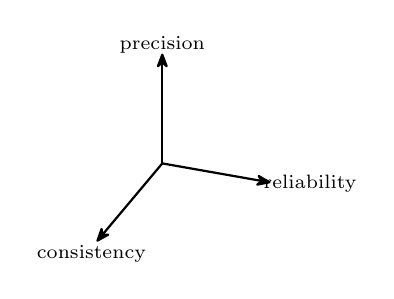
\begin{tikzpicture}
      \draw[flow, shorten <=0pt] (0,0) -- (0,1.5) node[font=\scriptsize]{precision};
      \draw[flow, shorten <=0pt] (0,0) -- ++(-10:1.5cm) node[font=\scriptsize, xshift=0.4cm]{reliability};
      \draw[flow, shorten <=0pt] (0,0) -- ++(230:1.4cm) node[font=\scriptsize, yshift=-2pt]{consistency};
    \end{tikzpicture}
    \begin{description}
      \item[Precision] \texttt{parallax\_error}, \texttt{pmra\_error}, \texttt{pmdec\_error}, etc
        \hfill $\longrightarrow$ OK \hskip1cm\null
      \item[Reliability] \texttt{visibility\_periods\_used} ($\geq6$ for 5-parameter solutions)
        \hfill $\longrightarrow$ OK \hskip1cm\null
      \item[Consistency] (goodness of fit to the 5-parameter model)
        \begin{equation*}
          \left .
          \begin{gathered}
            \text{\tt astrometric\_n\_bad\_obs\_al} \hfill \\
            \text{\tt astrometric\_gof\_al} \hfill \\
            \text{\tt astrometric\_chi2\_al} \hfill \\
            \text{\tt astrometric\_excess\_noise} \hfill \\
            \text{\tt astrometric\_excess\_noise\_sig}  \hfill
          \end{gathered}\quad
        \right \} \quad \longrightarrow \text{not recommended}
        \end{equation*}
    \end{description}
  \end{center}
\end{agaframe}
%
%%%%%%%%%%%%%%%%%%%%%%%%%%%%%%%%%%%%%%%%%%%%%%%%%%%%%%%%%%%%%%%%%%%%%%%%%%%%%
%
\begin{agaframe}{Renormalized Unit Weight Error}
  \begin{itemize}
    \item Recommded GoF indicator for Gaia DR2 astrometry
      \begin{itemize}
        \item Not given directly in the Gaia archive
      \end{itemize}
    \item Can be computed from the quantities:
      \begin{align*}
        \chi^2 & = \text{\tt astrometric\_chi2\_al} \\
        N & = \text{\tt astrometric\_n\_good\_obs\_al} \\
        G & = \text{\tt phot\_g\_mean\_mag} \\
        C & = \text{{\tt bp\_rp} (if available)}
      \end{align*}
    \item Unit weight error $\text{UWE} = \sqrt{\chi^2/(N-5)}$
    \item Renormalized unit weight error $\text{RUWE}=\text{UWE}/u_0(G,C)$
    \item $u_0(G,C)$ is an empirical normalization factor, provided as a lookup table on the ESA
      Gaia DR2 \href{https://www.cosmos.esa.int/web/gaia/dr2-known-issues}{Known Issues} pages
      \begin{itemize}
        \item A separate function $u_0(G)$ is provided for sources without a known colour
      \end{itemize}
    \item Python code to calculate RUWE: \url{https://github.com/agabrown/gaiadr2-ruwe-tools}
  \end{itemize}
\end{agaframe}
%
%%%%%%%%%%%%%%%%%%%%%%%%%%%%%%%%%%%%%%%%%%%%%%%%%%%%%%%%%%%%%%%%%%%%%%%%%%%%%
%
\begin{agaframealt}{Normalization factor $u_0(G,C)$}{Normalization factor}
  \begin{center}
    \begin{tikzpicture}
      \node (fig)
      {\includegraphics[height=6cm]{UseOfGaiaAstrometry/Lindegren_RUWE_normalizationfactor.png}};
      \node at ($(fig.south east)+(0,1)$) [anchor=south west, font=\tiny] {Figure: L.~Lindegren};
    \end{tikzpicture}
  \end{center}
  
  \medskip
  This is essentially the `typical' UWE for a given magnitude and colour
\end{agaframealt}
%
%%%%%%%%%%%%%%%%%%%%%%%%%%%%%%%%%%%%%%%%%%%%%%%%%%%%%%%%%%%%%%%%%%%%%%%%%%%%%
%
\begin{agaframe}[1-2]{Illustration of the use of RUWE}
  \only<1>{
    \begin{tikzpicture}
      \node (fig)
      {\includegraphics[height=7cm]{UseOfGaiaAstrometry/Lindegren_HRD_100pc_noUWEorRUWEfilter.png}};
      \node at ($(fig.north east)+(-0.5,-0.7)$) [anchor=north east, font=\tiny] {Figure: L.~Lindegren};
      \node at (fig.east) [anchor=west, text width=7cm, text badly ragged] {
        Selection:
        \begin{itemize}
          \item $\varpi>10$~mas
          \item $\varpi/\sigma_\varpi>10$
          \item Signal to noise in BP and RP larger than 10
          \item No filtering on goodness of fit indicators
        \end{itemize}
      };
    \end{tikzpicture}
  }
  \only<2>{
    \begin{tikzpicture}
      \node (fig)
      {\includegraphics[height=6cm]{UseOfGaiaAstrometry/Lindegren_HRD_100pc_UWEvsRUWEfilter.png}};
      \node at ($(fig.north)+(-0.5,-0.7)$) [anchor=north east, font=\tiny] {Figures: L.~Lindegren};
      \node at (fig.south) [anchor=north, text width=14cm, text badly ragged] {
        \begin{itemize}
          \item Filtering by RUWE gives cleaner HRD
          \item Blue dots are sources missing in left diagram
          \item Experiment to decide on the limit in RUWE for your application!
        \end{itemize}
      };
    \end{tikzpicture}
  }
\end{agaframe}
%
%%%%%%%%%%%%%%%%%%%%%%%%%%%%%%%%%%%%%%%%%%%%%%%%%%%%%%%%%%%%%%%%%%%%%%%%%%%%%
%
\begin{agaframe}{Example of quality cuts customized for M/L dwarf sample}
  \begin{tikzpicture}
    \node (cmd) {\includegraphics[height=6.5cm]{UseOfGaiaAstrometry/KimanEtAl_GabsvsG_RP_full.png}};
    \node at (cmd.south) [anchor=north, text width=5.5cm, text badly ragged, font=\scriptsize] {
      CMD with M/L dwarf sample after quality cuts described in
      \href{https://arxiv.org/abs/1904.05911}{Kiman et al.\ (2019, arXiv:1904.05911)}
    };
    \node (uwe) at (cmd.north east) [anchor=north west] {\includegraphics[height=2cm]{UseOfGaiaAstrometry/KimanEtAl_u_vs_G.png}};
    \node (fluxsnr) at (uwe.south west) [anchor=north west]
    {\includegraphics[height=2cm]{UseOfGaiaAstrometry/KimanEtAl_flux_over_errorvsmagnitude.png}};
    \node at (fluxsnr.south west) [anchor=north west, text width=8.0cm, text badly ragged]{
      \begin{itemize}
        \item Lindegren et al.\ (2018) cuts on UWE and photometric quality too conservative for M/L
          dwarfs
          \begin{itemize}
            \item UWE cuts were not designed with specific source colours in mind
            \item these stars are very red and thus expected to have low \gbp\ SNR
          \end{itemize}
      \end{itemize}
    };
  \end{tikzpicture}
\end{agaframe}
%
%%%%%%%%%%%%%%%%%%%%%%%%%%%%%%%%%%%%%%%%%%%%%%%%%%%%%%%%%%%%%%%%%%%%%%%%%%%%%
%
\begin{agaframe}[1-2]{Ingredients of Gaia DR2 selection function}
  \only<1>{
    \begin{tikzpicture}
      \node (fpa) {\includegraphics[height=4.5cm]{FocalPlanes/FocalPlaneKohley.png}};
      \node (windows) at (fpa.north east) [anchor=north west]
      {\includegraphics[height=4.0cm]{DataProcessing/GaiaViewOfR136_20110622-outsidecore.png}};
      \node at (windows.south) [anchor=north, font=\tiny] {Credits: ESA/R.~Kohley/J.~de~Bruijne};
    \end{tikzpicture}
    \begin{itemize}
      \item Detection of sources in SM1/2, confirmation in AF1 (as cosmic ray/ spurious source
        rejection step)
      \item Strict flux threshold applied, but in presence of magnitude estimation errors
      \item Limit on source `size'
      \item Management of observation window conflicts and resource limitations affects completeness
        in crowded fields (above few 100k stars/degree$^2$)
      \item Details in \href{https://doi.org/10.1051/0004-6361/201629272}{Gaia Collaboration, Prusti
        et al.}, \href{https://doi.org/10.1051/0004-6361/201424018}{de Bruijne et al.}
    \end{itemize}
  }
  \only<2>{
    \begin{tikzpicture}
      \node (skymap) {\includegraphics[height=4.3cm]{GaiaDR2/Contents/RVS_dr2_Maps_All_counts_hp07.png}};
      \node at (skymap.north) [anchor=south, font=\scriptsize] {RVS Source counts (Katz et al.~2019)};
      \node (completeness) at (skymap.east) [anchor=west]
      {\includegraphics[height=4.3cm]{GaiaDR2/Contents/Completeness_G_99th_percentile.png}};
      \node at (completeness.north) [anchor=south, font=\scriptsize] {99th percentile in $G$ (Arenou
      et al.~2018)};
    \end{tikzpicture}
    \begin{itemize}
      \item Imprints from Initial Gaia Source List in RVS counts (will disappear in future)
      \item Brighter magnitude limit in crowded fields
      \item Imprint of combination of scan law pattern and data quality filtering
      \item Knock-on effects of data quality filtering during data processing (also follows scan
        law)
    \end{itemize}
  }
\end{agaframe}
%
%%%%%%%%%%%%%%%%%%%%%%%%%%%%%%%%%%%%%%%%%%%%%%%%%%%%%%%%%%%%%%%%%%%%%%%%%%%%%
%
\begin{agaframe}{Epoch propagation and cross-matching to other catalogues}
  \begin{itemize}
    \item Gaia DR2 has high spatial resolution, down to $0.4$--$0.5$ arcsec (PSF is $\sim0.1$
      arcsec)
      \begin{itemize}
        \item most other catalogues are of lower resolution so beware of blended sources
      \end{itemize}
    \item Gaia DR2 reference epoch is 2015.5
      \begin{itemize}
        \item propagate Gaia positions to epoch of other catalogue before doing positional match
        \item requires proper motions (and parallax and radial velocity for rigorous treatment)
          \begin{itemize}
            \item if not available use proper motion dispersion for the source population being
              matched to estimate positional uncertainties at other epoch
          \end{itemize}
        \item reference system for modern catalogues is ICRS; no need to worry about precession,
          nutation, etc
        \item all maths, including propagation of covariance matrix, in Gaia DR2 online documentation
        \item see
          \href{http://docs.astropy.org/en/stable/api/astropy.coordinates.SkyCoord.html}{\texttt{astropy.coordinates.SkyCoord.apply\_space\_motion()}}
      \end{itemize}
    \item Pre-computed cross-matches to large catalogues available from Gaia archive
      \begin{itemize}
        \item these are carefully done positional matches, not necessarily complete
        \item details in \href{https://doi.org/10.1051/0004-6361/201834142}{Marrese et al.}
      \end{itemize}
    \item Convenient tools offered by \href{http://www.star.bris.ac.uk/~mbt/topcat/}{Topcat} and \href{http://cdsxmatch.u-strasbg.fr/}{CDS x-match service}
  \end{itemize}
\end{agaframe}
%
\end{document}
